\chapter{Study}
\label{chapter3}

\section{Approach}

In order to measure the method coverage reached by an exploration tool in one application, there is the need to know how many methods there are in the application and how many methods were called during the exploration. To achieve that, the application developers could count the number of methods in their project and write log lines at the beginning of every method. After that, they will need to compile, run the exploration tool against their application, measure the number of methods that were called during the exploration and compute statistics.

With that in mind, this study consists of nearly the same stages, i. instrumentation, ii. exploration, iii. coverage analysis, iv. summarize, and v. compute statistics. The stages ii. and iii. were repeated 10 times for every application that was selected, that leaded to the iv. stage.

The different stages were completed as follow:

Stage i: 

The applications' instrumentation was made by using InstruAPK. It is an instrumentation tool developed mainly for this study. This tool uses APKTool, a known Java application that allows inverse engineering in Android apps, allowing applications' instrumentation without the need of recompiling their source code. APKTool decodes the apk and the result is the smali representation of the app source code, These smali files are analysed in order to find all the methods to be instrumented and then, the log code is injected at the very beginning of each method. Its important to notice that no external libraries methods are instrumented. InstruAPK only search for methods following the android project structure that uses the application package name to store the application source code.

Stage ii: 

The exploration was made by four different automatic exploration tools. two from the industry and two from the academic side. The first tool was Firebase Test Lab. it was selected for being widely used in industry and for also being a Google product. The second one, Monkey, was selected for being the most basic one and because it is also included in the SDK for developing Android Apps. The third one, Droidbot, was selected from the academic side. Droidbot has been a point of study for many researches. Many others tools have based their functionality on this tool. The last one is RIP, this tool was selected for being of special interest for us. It is our own exploration tool and is is currently an active project inside the Software Design Lab at University of Los Andes. 

Every tool was executed ten times per application, and every execution with a maximum time of 30 minutes. Some tools ended its exploration before the max time. 
The number of executions and the maximum time were arbitrary decisions that were made because of time limitations for the study. Although, during the study was notice that most of the tools ended the exploration or reached their maximum coverage within the first 15 minutes. Which means that the maximum time for exploration was more than enough in almost all cases. 
 
stage iii: 

The coverage measurement was made by CoverageAnalyzer. It is a Java Application created mainly for this study. It was made to analyse the resulting logcat of an Android phone, when executing an application that was instrumented by InstruAPK. It extracts different data such as, number of methods called, number of  methods never called, number of error traces of the application being analysed, most called methods, less called methods, as well as the time stamp of all calls of every method. It is important to notice that the possibility of extracting all those information is because InstruAPK provides it.

stage iv. 


\section{Approach Architecture}

\textbf{RIP Tests Generator} genera tests después de que \textbf{RIP} termina la ejecución, lo que permite el desacoplamiento de las dos herramientas. En este caso, \textbf{RIP} \cite{LinanAutomatedApps} puede mejorar o cambiar sus algoritmos de exploración dinámica sobre aplicaciones móviles, manteniendo la compatibilidad con \textbf{RIP Tests Generator}. La figura \ref{procesoTests} presenta el resumen del proceso de generación de tests a partir de los archivos obtenidos mediante la ejecución de RIP.

\begin{figure}[h]
	\centering
	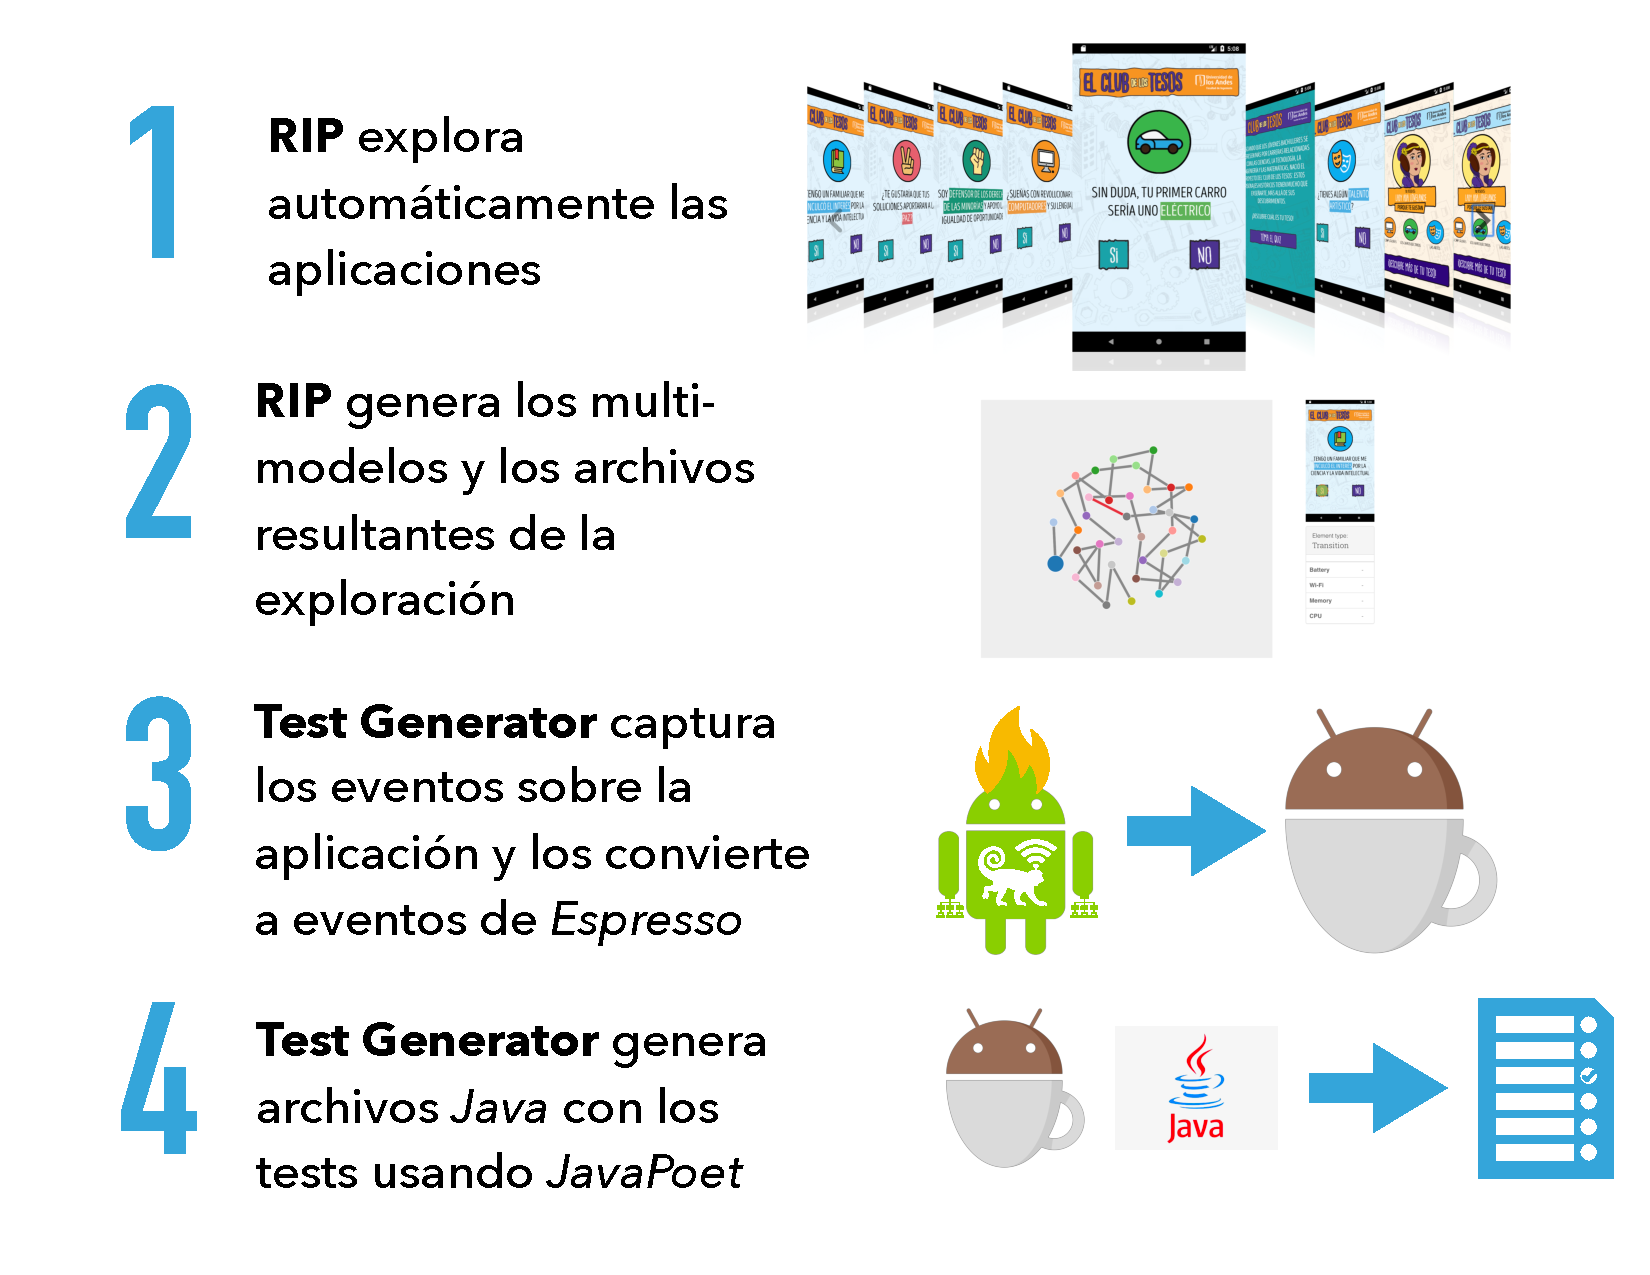
\includegraphics[width=1\textwidth]{img/procesoTests.pdf}
	\vspace{-0.5cm}
	\caption{Proceso de generación automática de tests}
	\label{procesoTests}
\end{figure} 

Test Generator es un componente acoplado con RIP que es ejecutado cuando se termina la exploración de la aplicación. Para esto, se creó la clase TestCaseBuilder.java que toma los datos proporcionados en el archivo tree.json y traduce los eventos a comandos de espresso.


Para la generación de pruebas se definieron los siguientes eventos, basados en los generados por RIP:

\textbf{TAP} : Cuando se tiene esta acción se traduce a un evento de hacer click en el botón o campo con el id proporcionado. Para implementar esta acción en espresso, se utiliza el comando \textit{onView(withId(id)).perform(click())}.

\textbf{INPUT} :  Al detectar un evento de campo de texto, con ayuda del modelo de dominio se detecta el tipo de dato a ingresar. Para esto se tiene la posibilidad de crear texto de manera aleatoria en un rango de caracteres normal o con una gran cantidad de estos con el fin de probar los limites de estos campos. Esta acción es implementada mediante el comando \textit{onView(withId(id)).perform(replaceText("randomtext"),closeSoftKeyboard());}



\section{Requisitos técnicos para la generación automática de pruebas}
Con el fin de que el desarrollador no tenga ningún inconveniente usando la herramienta, se definieron los siguientes requisitos técnicos:
\begin{enumerate}
	\item Al estar integrada con \textbf{RIP}\cite{LinanAutomatedApps}, se debe tener instalado ADB y correr el software en dispositivos rooteados o emuladores.
	\item El desarrollador debe tener acceso al código fuente de la aplicación, ya que los archivos de prueba generados solo pueden ser ejecutados si son empaquetados junto al código fuente.
	\item Es necesario htreeacer los cambios pertinentes en el build.gradle del proyecto para importar las dependencias utilizadas en los casos de prueba. Un ejemplo de esto es encontrado en la figura \ref{dependencies}.
	

\end{enumerate} 

	\begin{figure}[h]
	\centering
	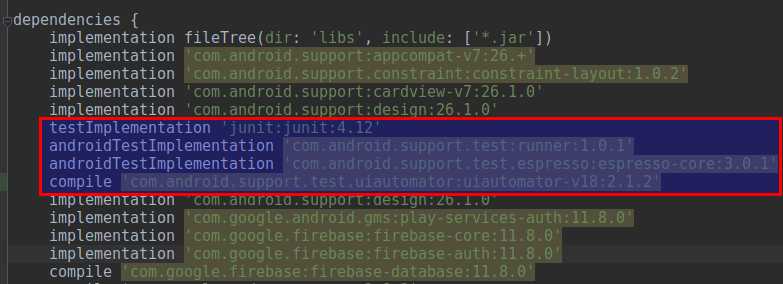
\includegraphics[width=1\textwidth]{img/dependencies.png}
	\vspace{-0.5cm}
	\caption{Ejemplo de archivo build.gradle con las dependencias necesarias para la ejecución de las pruebas}
	\label{dependencies}
\end{figure} 


\section{Generación automática de una prueba}
Para generar una prueba se hace uso del archivo tree.json \textbf{RIP}, el cual contiene un grafo donde las actividades corresponden a los nodos y los links a los eventos que disparan una transición entre dos estados. Cada nodo contiene la información del modelo de dominio con el tipo de datos que se encuentran. Además, se tienen los diferentes indicadores de contexto en cada estado, donde se pueden ver datos como batería, conectividad de internet, etc.

Dicho archivo es el que se utiliza como insumo para generar los casos de prueba mediante RIP Tests Generator. Gracias a la librería JavaPoet \cite{JavaPoet} se genera un archivo .java que contiene el código fuente de la prueba. Para esto, se tiene en cuenta la información obtenida del grafo generado por RIP y se hace una traducción de cada acción a ser ejecutada en la prueba.

Mediante el modelo GUI se pueden generar los eventos de transición. Por ejemplo, si la acción que produjo un cambio de estado es un tap en el botón con id 'buttonJugar', entonces esto será traducido como un \textit{onView(withId(R.id.buttonJugar)).perform(click());}. Para generar esto, se tiene un método auxiliar que retorna la línea de código correspondiente. Al analizar el grafo, según el tipo de acción encontrada se genera una línea de código diferente. Este proceso se puede evidenciar en el ejemplo de la figura \ref{gentest}.

Respecto a la implementación de la generación de código con JavaPoet se debe mencionar que las librerías correctamente declaradas son importadas de manera automática en el archivo generado. Además, el paquete donde debe ser ubicado el archivo fuente se inserta de manera correcta. Finalmente, después de cada acción, se toma una captura de pantalla que será posteriormente extraída del dispositivo para generar el reporte de visualización web.

El algoritmo propuesto para la generación de la prueba es el siguiente:

\begin{enumerate}
	\item Tomar la secuencia de eventos generada por RIP y guardarlos en una lista.
	\item Realizar la acción de tomar una captura de pantalla antes de cada transición.
	\item Según cada evento generar la línea de código correspondiente en el lenguaje espresso.
	\item Si se tiene un cambio de contexto en el nodo, realizar la traducción correspondiente.
	\item Con la ayuda de JavaPoet, generar los campos usados por Espresso. Como lo son la ActivityTestRule, para indicar en que actividad iniciar la aplicación, y los permisos de escritura y lectura para las capturas de pantalla.
	\item Finalmente, para la correcta ejecución de la prueba, se genera un archivo ejecutable que se encarga de empaquetar el apk, correr las pruebas encontradas en el paquete test, y extraer las capturas de pantalla del dispositivo.
\end{enumerate}
Un ejemplo de la prueba obtenida como resultado puede ser evidenciado en la figura \ref{pruebaresultado}

\begin{figure}[h]
	\centering
	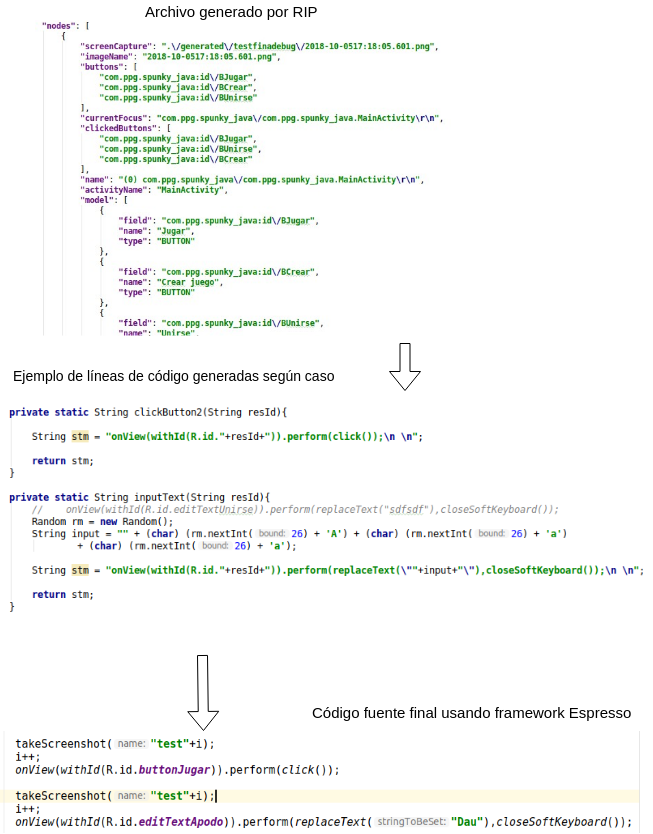
\includegraphics[width=1\textwidth]{img/GeneracionPrueba.png}
	\vspace{-0.5cm}
	\caption{Proceso de traducción y generación de prueba}
	\label{gentest}
\end{figure} 

\begin{figure}[h]
	\centering
	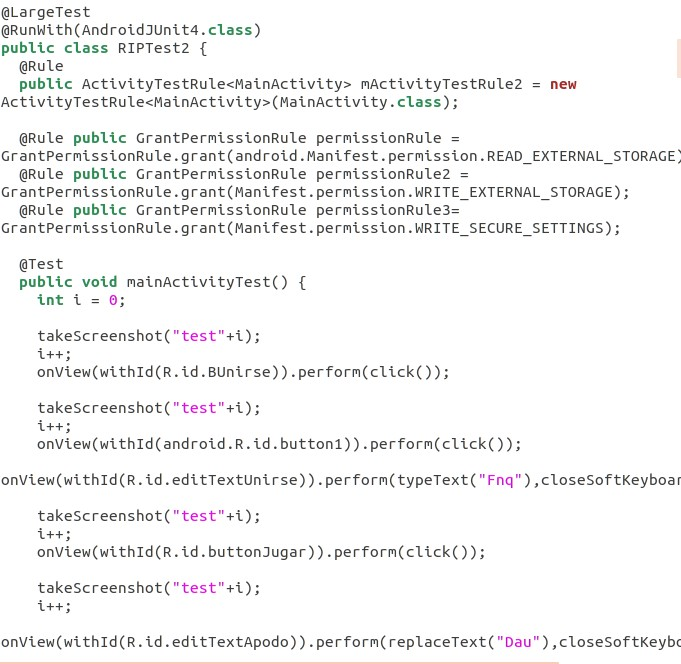
\includegraphics[width=1\textwidth]{img/pruebaResultado.jpg}
	\vspace{-0.5cm}
	\caption{Prueba generada}
	\label{pruebaresultado}
\end{figure} 







	
